\documentclass[12pt, twoside]{article}
\usepackage[letterpaper, margin=1in, headsep=0.5in]{geometry}
\usepackage[english]{babel}
\usepackage[utf8]{inputenc}
\usepackage{amsmath}
\usepackage{amsfonts}
\usepackage{amssymb}
\usepackage{tikz}
\usepackage{yhmath}
%\usetikzlibrary{quotes, angles}

\usepackage{graphicx}
\usepackage{enumitem}
\usepackage{multicol}

\usepackage{fancyhdr}
\pagestyle{fancy}
\fancyhf{}
\renewcommand{\headrulewidth}{0pt} % disable the underline of the header

\fancyhead[RE]{\thepage}
\fancyhead[RO]{\thepage \\ Name: \hspace{3cm}}
\fancyhead[L]{BECA / Dr. Huson / 10th Grade Geometry\\* 15 May 2019}

\begin{document}
\subsubsection*{11.3 Homework: Compound shapes and their volumes}
 \begin{enumerate}

   \item A wooden board is cut square at one end and at a $45^\circ$ angle at the other. Overall it is 8 feet long, 12 inches wide, and 2 inches thick.\\[0.5cm]
   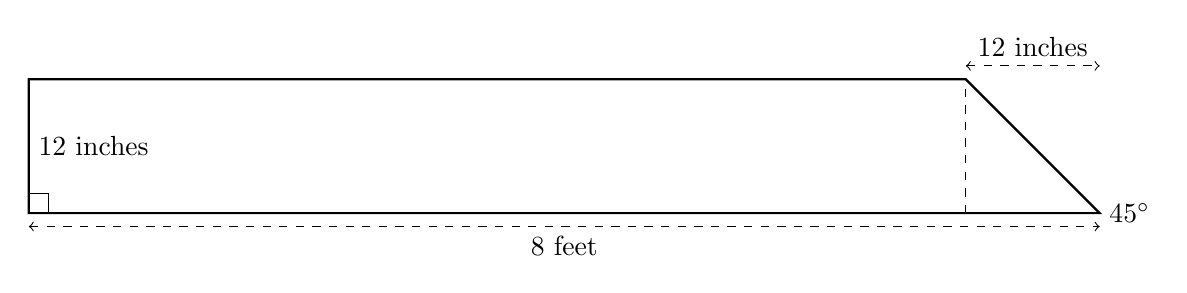
\begin{tikzpicture}[scale=1.7]
     \draw [thick]
     (0,0)--(0,1)--(7,1)--(8,0)--cycle;
     \draw [dashed] (7,0)--(7,1);
     \draw [dashed,<->] (7,1.1)--(8,1.1);
     %\draw [->] (45:0.5)--(45:0.9142);
     %\draw [->] (45:2.3)--(45:1.9142);
     \draw (0,0)++(0,0.15)--++(0.15,0)--+(0,-0.15);
     \draw [dashed,<->] (0,-0.1)--(8,-0.1);
     \node at (4,-0.1)[below]{$8 \ \mathrm{feet}$};
     \node at (0,0.5)[right]{$12 \ \mathrm{inches}$};
     \node at (7.5,1.1)[above]{$12 \ \mathrm{inches}$};
     \node at (8,0)[right]{$45^\circ$};
   \end{tikzpicture} \vspace{0.5cm}

   \begin{enumerate}
     \item Determine and state the volume of the board to the \emph{nearest  cubic inch}. \vspace{9cm}
     \item Find the weight of the board, to the \emph{nearest pound}. Use 44 lbs/ft$^3$ for the density of wood.
   \end{enumerate}

\newpage
   \item New streetlights will be installed along a section of the highway. The posts for the streetlights will be 7.5 m tall and made of aluminum. The city can choose to buy the posts shaped like cylinders or the posts shaped like rectangular prisms. The cylindrical posts have a hollow core, with aluminum 2.5 cm thick, and an outer diameter of 53.4 cm. The rectangular-prism posts have a hollow core, with aluminum 2.5 cm thick, and a square base that measures 40 cm on each side.\\[0.25cm]
   Sketch the two shapes (cylinders \& rectangular prisms), and calculate their volumes.\\[8cm]
   The density of aluminum is 2.7 g/cm$^3$, and the cost of aluminum is \$0.38 per kilogram.\\[0.25cm]
   If all posts must be the same shape, which post design will cost the town less?\\[5cm]

   How much money will be saved per streetlight post with the less expensive design?

\end{enumerate}
\end{document}
